\documentclass{article}
\textheight 23.5cm \textwidth 15.8cm
%\leftskip -1cm
\topmargin -1.5cm \oddsidemargin 0.3cm \evensidemargin -0.3cm
%\documentclass[final]{siamltex}

\usepackage{ctex}
\usepackage{verbatim}
\usepackage{fancyhdr}
\usepackage{graphicx}
\usepackage{amsmath}
\usepackage{amssymb}
\usepackage{float}
\usepackage{multirow}
\usepackage{colortbl}
\usepackage{amsthm}
\usepackage{bm}
\usepackage{tikz}

\textheight 23.5cm \textwidth 15.8cm
\topmargin -1.5cm \oddsidemargin 0.3cm \evensidemargin -0.3cm
\title{HW10 实验报告}
\author{PB20010429 侯相龙}

\begin{document}
\maketitle
\section{实验内容}
实现平行投影


\section{实验原理}
利用Homogeneous坐标,正交(平行)投影和透视投影的矩阵为:
\begin{description}
    \item[正交投影:] 假设原立方体大小为$[l,r]\times[b,t]\times[f,n]$。则正交投影矩阵为:
    \begin{equation}\label{eq1}
        \mathbf{M}_{orth}=\begin{bmatrix}\frac{2}{r-l}&0&0&-\frac{r+l}{r-l}\\ 0&\frac{2}{t-b}&0&-\frac{t+l}{t-b}\\ 0&0&\frac{2}{n-f}&-\frac{n+f}{n-f}\\ 0&0&0&1\end{bmatrix}
    \end{equation}
    \item [透视投影]近远平面不动,远平面中心不动,对视锥体进行挤压。先挤成正交投影的长方体,后用正交投影的方式进行投影。
    \begin{figure}[h]
        \begin{center}
            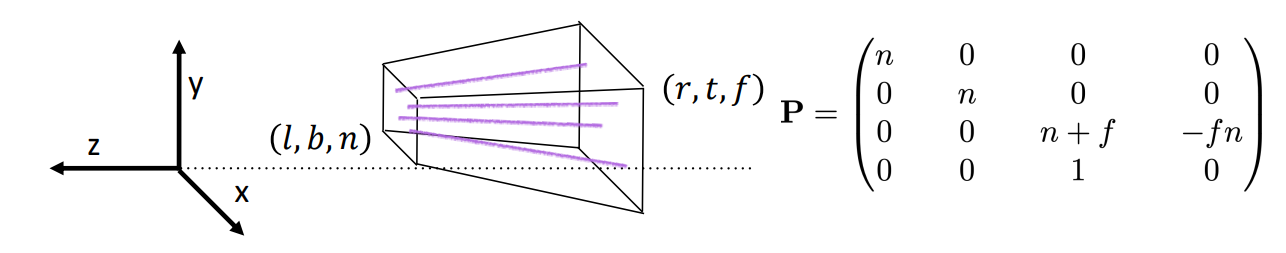
\includegraphics[width=0.7\linewidth]{2.png}
        \end{center}
        \caption{透视投影及投影矩阵}
    \end{figure}
\end{description}

\section{算法介绍与步骤}
按\ref{eq1} 构建矩阵即可


\section{实验结果}

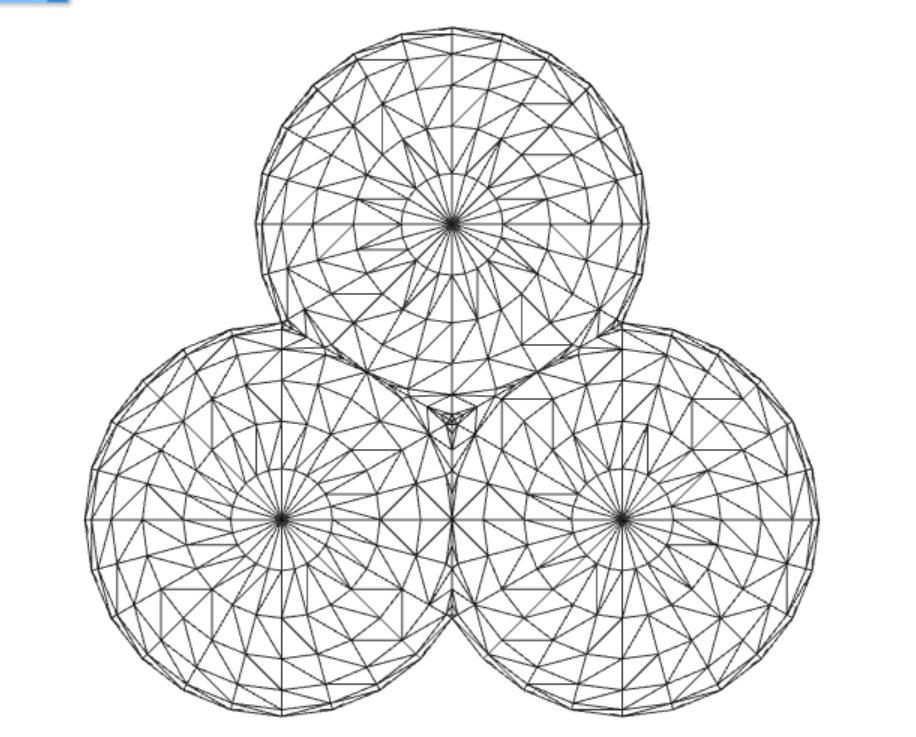
\includegraphics[width=0.7\linewidth]{1.png}

对比原投影效果,平行投影灯中心点在圆心无偏移



\end{document}
